\label{app:relaxed}

The relaxed memory model is a fragment of RC20 memory model,  introduced by Margalit and Lahav 2021 \cite{Margalit:2021} which defines a rich fragment of the C11 model consisting of acquire/release and relaxed accesses.  Consistency testing for $\rlxmm$ is known to be polynomial time when number of threads, variables and values are fixed. But for the stronger version of $\rlxmm$ where \PORF{} is allowed, the problem becomes NP-Complete \cite{ChakrabortyKMP24}. Please refer to Table~\ref{table:ax:models-2-app} for the axioms for $\rlxmm$-Acyclic. 
In this chapter, we study the complexity of the $\vm$- problem for both the `Relaxed' and the 'Relaxed-Acyclic' fragment of C-11. Relaxed model satisfy the coherence axioms: \RlxRCoh{} and \RlxWCoh{}  (Table~\ref{table:ax:models-2-app}). Essentially all $\hb$'s in \WRCoh{} and \WCoh{} are replaced by $\po$.  Figure~\ref{fig:relaxed-illust-app} recalls the instances for violation of the relaxed axioms.     The overview of this chapter is as follows:
\begin{itemize}
 \item Section~\ref{sec-onewriter-relaxed} gives a  $\mathcal{O}(n^3)$ algortihm for the $\vm$-problem restricted to  \onewriter~ under $\rlxmm$-Acyclic memory model.
 
 \item Section~\ref{sec:finegrained-relaxed} gives a conditional lower bound of $2^{o(k)}\dot n^{O(1)}$ under ETH for the $\vm$-problem restricted to  \threewriter.
 
 \item Section~\ref{sec:np-relaxed} shows that the $\vm$-problem restricted to \twowriter~ is NP-Complete.
\end{itemize}

\begin{table}
    \caption{\small Coherence Axioms for $\rlxmm$-Acyclic variant of C11}
    \label{table:ax:models-2-app}
    \centering
    %\small
    \begin{tabular}{lr}
   % \multicolumn{2}{c}{\underline{Release-Acquire}} \\
    %$\irr(\mo_x;\hb)$ & (\WCoh{})\\
    %$\acy(\hb \cup \mo)$ & (\SWCoh{})\\
    %$\irr(\rf^{-1};\mo_x;\hb)$ & (\RCoh{})\\
    %$\irr(\hb_x;[\W];\hb_x;\rf^{-1})$ & (\WRCoh{})\\
    %\hline
    \multicolumn{2}{c}{\underline{Relaxed-Acyclic}} \\
    $\irr(\po\cup\rf)$ & (\PORF{})\\
    $\irr(\mo_x;\po)$ & (\RlxWCoh{})\\
    $\irr(\rf^{-1};\mo_x;\rf^?;\po)$ & (\RlxRCoh{})\\
    \end{tabular}
\end{table}
The next section contains the PTIME-algorithm for $\onewriter$ systems along with its proof of correctness and complexity. The hardness results with relevant theorems will be presented in the following sections. 
\iffalse
\begin{table}
     \caption{\small The C11 models $\wramm, \ramm, \sramm, \rlxmm$.}
    \label{table:ax:models-2-app}
     
        \setlength\tabcolsep{7.5pt}
      \begin{tabular}{lr|lr}
      \multicolumn{2}{l|}{} & \multicolumn{2}{l}{} \\
      $\wramm$ & \makecell{\PORF{}\\ \WRCoh{}} &$\rlxmm$ & \makecell{\PORF{}\\ \RlxRCoh\\ \RlxWCoh} \\ 
      \hline
      $\ramm$ & \makecell{\PORF{} \\
      \WCoh{}\\ \RCoh{}}   &$\sramm$ & \makecell{\PORF{}\\ \SWCoh{}\\ \RCoh{}}\\ 
      \cline{1-4}
      %$\sramm$ & \makecell{\SWCoh{}\\ \RCoh{}} & & \\ 
      \end{tabular}
          
  \end{table}
\fi
 \begin{figure}[t]
    \def\ystep{0.4}
    \centering
     \resizebox{0.5\textwidth}{!}{
	\begin{tikzpicture}[yscale=1]
	
      \node (t11) at (12.3,0*\ystep)  {$\wt_1(x)$};
      \node (t12) at (12.3,-4*\ystep) {$\wt_2(x)$};
      \node (t0) at (12.3,-5*\ystep) {$(a)$};
      \draw[mo] (t12) to[bend left=45] node[left]{$\mo$} (t11);
    %  \draw[po] (t12) to (t13);
    %  
      \draw[po] (t11) to (t12);
    %%%%%%%%%%%%%%%%%%%%%%%%%%%%%%%%%%%%%%%%%%%%%%%%%%%%%%%%%%%%%%%%%%%%%%%%%%%%%%%%%
     \node (t11) at (16.3,0*\ystep)  {$\wt_1(x)$};
      \node (t12) at (16.3,-4*\ystep) {$\wt_2(x)$};
    %  \node (t13) at (0,-4.5*\ystep) {$\rd(x)$};
    %
      \node (t21) at (18.1,0*\ystep) {$\rd_2(x)$};
      \node (t22) at (18.1,-4*\ystep) {$\rd_1(x)$};
      \node (t1) at (17.2,-5*\ystep) {$(b)$};
    %
      \draw[mo] (t11) to node[left]{$\mo$} (t12);
    %  \draw[po] (t12) to (t13);
    %  
      \draw[po] (t21) to (t22);
    %  \draw[po] (t22) to (t23);
    %
    %  \draw[rf,bend left=0] (t11) to node[below,pos=0.9, sloped]{$\rf$} (t23);
    %  \draw[rf,bend right=0] (t21) to node[below,pos=0.9, sloped]{$\rf$} (t13);
    %    
      \draw[rf,bend left=0] (t12) to node[above, pos=.8, sloped]{$\rf$}(t21);
      \draw[rf,bend right=0] (t11) to node[below,pos=0.8, sloped]{$\rf$} (t22);
    
    \end{tikzpicture}
	 }
    \caption{Violation of (a)~\RlxWCoh:$\wt_2(x)~\mo~\wt_1(x), \wt_1(x)~\po~\wt_2(x)$ (b)~\RlxRCoh{}: $\wt_1(x)~\mo~\wt_2(x)$, $\rd_2(x)~\po~\rd_1(x)$ 
      with $\wt_2(x)~\rf~\rd_2(x)$ and $\wt_1(x)~\rf~\rd_1(x)$.}
      \label{fig:relaxed-illust-app}
\end{figure}



\section{Polynomial Time for \onewriter\ systems}\label{sec-onewriter-relaxed}
Here we give a polynomial time algorithm for solving  the $\vm$-problem for \onewriter~ under $\rlxmm$-Acyclic memory model. Note that as $\rlxmm$-Acyclic is stronger than $\rlxmm$, any polynomial time result for $\rlxmm$-Acyclic would also hold for $\rlxmm$.
As for \onewriter~ systems we have $\mo=\po$, \RlxWCoh{} would always hold. Hence to show that an execution graph $\expartial$ is $\rlxmm$-Acyclic-consistent, we need to verify \PORF{} and \RlxRCoh{}. We can state the following lemma for $\rlxmm$-Acyclic similar to  Lemma~\ref{lem:onewriter-axioms-two-properties} of Chapter~\ref{RA-ptime}. For $\rlxmm$, as \PORF{} is not required, only the second part of the lemma is meaningful and proof is same.

\begin{restatable}{lemma}{lemmaonewriterrelaxedtwoproperties-relaxed}
    \label{lem:relaxed-onewriter-axioms-two-properties}
Let $\rf_1$ and $\rf_2$ be two reads-from functions over a partial \onewriter\ execution graph $\ex=(\E, \po, \mo)$ s.t. $\mo$ agrees with $\po$. 
\begin{itemize}
\item Suppose $\rf_1 \sqsubseteq \rf_2$. Then, if $\rf_1$ induces a $\po \cup \rf_1$ cycle, then $\rf_2$ induces a $\po \cup \rf_2$ cycle.
\item Suppose both $\rf_1$ and $\rf_2$ satisfy relaxed-read-coherence. Then, the $\rf$ function $\min(\rf_1, \rf_2)$ also satisfies relaxed-read-coherence.
\end{itemize} 
\end{restatable}
\begin{proof}
 The proof for the first part is same as that of $\wramm$ in lemma~\ref{lem:onewriter-axioms-two-properties} and hence we skip it.
 
 For the second part, we denote $\rf_0=min(\rf_1,\rf_2)$. We shall show that that if $\rf_0$ violates relaxed-read-coherence, then either $\rf_1$ or $\rf_2$ violates it. Suppose $\rf_0$ induces a violation of relaxed-read-coherence. There is a cycle of the form:
 \[ r \xra{\rf_0^{-1}} w \xra{\po^+} w' \xra{\rf_0} r' \xra{\po^+} r\], where all of $w,w',r$ and $r'$ are in the same variable.
 By definition, either $\rf_1$ or $\rf_2$ associates $r$ to $w$. WLOG, say $\rf_1(r) = w$. Then either $w'~\rf_1~r'$ or $w'~\rf_2~r'$. For the former case, $\rf_1$ is not $\rlxmm$-consistent. For the later case,  there is a write event $w^{''}$ on $\xvar$ such that $w'~\po^*~w{''}~\rf_1~r'$ as $\rf_0$ maps $r'$ to the $\po$-earlier read between $\rf_1(r')$ and $\rf_2(r')$. Again relaxed-read-coherence of $\rf_1$ fails thereby proving the second item. 
\end{proof}
Lemma~\ref{lem:relaxed-onewriter-axioms-two-properties} implies the existence of an unique minimum $\rf$ $\rf_{min}$ that satisfies \RlxRCoh{}. Thus $\rlxmm$-consistency testing  reduces to finding $\rf_{min}$. In case of $\rlxmm$-Acyclic-consistency testing, we also check for \PORF{}.

\begin{algorithm}[h!]
\caption{$\rlxmm$-Acyclic-consistency checking in \onewriter\ systems}
\label{algo:one-writer-relaxed}
\Fn{$\CheckC(\expartial)$}{
    $\rf \gets \Initialize(\expartial)$ \\
    \While{$\rf$ violates relaxed-read-coherence}{\label{algo-while-main-onewriter-relaxed}
        $\rf \gets \update(\expartial, \rf)$  \label{algo-update-call-relaxed}
    }
    \Comment{Now $\rf = \rf_{\min}$}
    \If{$\rf$ satisfies porf-acyclicity}{ \label{algo-check-porf-relaxed}
        \Return $\expartial$ is $\rlxmm$-Acycic-consistent \label{algo-declare-consistent-relaxed}
    }
    \Else {
        \Return $\expartial$ is not $\rlxmm$-Acyclic-consistent  \label{algo-porf-cycle-relaxed}
    }
}


\Fn{$\Initialize(\expartial)$}{
\For{each read $r = \rd(x, v)$}{
$t \gets$  thread containing $r$ \\
$t_x \gets$ writer thread for $x$ \\
\If{$t \neq t_x$}{
    $\rf^{-1}_0(r) \gets$ $\po$-smallest write $w$ of the form $\wt(x,v)$ in $t_x$ \\
    \If{there is no such write}{
        \Return $\expartial$ is not $\rlxmm$-Acyclic-consistent \label{init-not-consistent1-relaxed}
    }
}
\If{$t = t_x$}{
    $\rf^{-1}_0(r) \gets$ $\po$-smallest write $w$ of the form $\wt(x,v)$ in $t_x$ s.t. $w~\po^+r$ \\
    \If{there is no such write}{
        \Return $\expartial$ is not $\rlxmm$-Acyclic-consistent \label{init-not-consistent2-relaxed}
    }
}
}
\Return $\rf_0$
}

\Fn{$\update(\expartial, \rf_i)$}{
    Pick a cycle violating relaxed-read-coherence: $r_i \xra{\rf_i^{-1}} w_i \xra{po} w'_i \xra{\rf} r'_i \xra{po} r_i$ \label{algo-violatecycle-relaxed} \\
    Let $r_i = \rd(x, v)$, $w_i = \wt(x, v)$, $w'_i = \wt(x, v')$ \\
    $t \gets$ thread of $r_i$ \\
    $t_x \gets$ writer thread of variable $x$ \\
    \If{$t \neq t_x$}{
    $\rf^{-1}_{i+1}(r_i) \gets$ $\po$-smallest write $w''_i$ of the form $\wt(x,v)$ in $t_x$ s.t. $w'_i ~\po^* w''_i$ \label{algo-update1-relaxed} \\
    \If{there is no such write}{
        \Return $\expartial$ is not $\rlxmm$-Acyclic consistent  \label{algo-update-notconsistent1-relaxed}
    }
}
\If{$t = t_x$}{
    $\rf^{-1}_{i+1}(r_i) \gets$ $\po$-smallest write $w''_i$ of the form $\wt(x,v)$ in $t_x$ s.t. $w'_i ~\po^* w''_i ~\po^+r_i$ \label{algo-update2-relaxed}\\
    \If{there is no such write}{
        \Return $\expartial$ is not $\rlxmm$-Acyclic-consistent \label{algo-update-notconsistent2-relaxed}
    }
}
$\rf^{-1}_{i+1}(r') \gets \rf_i(r')$ for all $r' \neq r_i$ \\
\Return $\rf_{i+1}$
}
\end{algorithm}

\textbf{Finding the smallest $\rlxmm$-Acyclic-consistent $\rf$} To show that an execution graph, $\expartial$ satisfies $\rlxmm$-Acyclic-consistency, we check for \PORF{} and \RlxRCoh{}. 

Algorithm~\ref{algo:one-writer-wra} in Chapter~\ref{RA-ptime}  can be modified to obtain a PTIME algorithm for $\rlxmm$ and $\rlxmm$-Acyclic. The modifications are as follows:
\begin{itemize}
 \item Any appearance of \WRCoh{} would be replaced  by \RlxRCoh{}.
 
 \item Any appearance of $\wramm$-consistency would be replaced by $\rlxmm$ ($\rlxmm$-Acyclic) consistency.
 
 \item Line~20 of Algorithm~\ref{algo:one-writer-wra} would be replaced by `Pick a cycle violating relaxed-read-coherence: $r_i \xra{\rf_i^{-1}} w_i \xra{po} w'_i \xra{\rf} r'_i \xra{po} r_i$. 
 
 \item We use check for \PORF{} in line~\ref{algo-check-porf} of Algorithm~\ref{algo:one-writer-wra} only if the underlying memory model is $\rlxmm$-Acyclic. For vanilla $\rlxmm$ memory model such check will be omitted.
 \end{itemize}
 
 The modified version for $\rlxmm$-Acyclic is presented as Algorithm~\ref{algo:one-writer-relaxed}. Note that, by construction of the algorithm, \RlxWCoh{} is never violated.  The correctness of the algorithm uses Lemma~\ref{lem:relaxed-onewriter-axioms-two-properties} and is analogous to that of Algorithm~\ref{algo:one-writer-wra}. Theorem for showing correctness of Algorithm~\ref{algo:one-writer-relaxed} is given below.

\begin{restatable}{theorem}{thmrlxcorrectness}\label{th-wra-correctness}
A partial execution graph $\expartial = (\E, \po)$ of a one-writer system is consistent for $\rlxmm$-Acyclic iff  Algorithm~\ref{algo:one-writer-relaxed} returns $\expartial$ is $\rlxmm$-Acyclic-consistent. Moreover, the algorithm runs in time $\mathcal{O}(n^3)$ where $n = |E|$  and returns the smallest $\rf$ function that is $\rlxmm$-Acyclic-consistent, if one exists.
\end{restatable}

\begin{proof}
Let $\rf_0$ be the initial $\rf$ function assigned by Line 2 of the algorithm. Notice that if $\Initialize$ executes either Line~\ref{init-not-consistent1-relaxed} or \ref{init-not-consistent2-relaxed}, then there is a read for which no write can be assigned, and hence there is no $\rf$ function at all, and there is nothing more to prove. Let us assume $\Initialize$ returns an $\rf$ function $\rf_0$. 

Let $\rf_i$ be the $\rf$ function assigned by the $i^{th}$ call to the $\update$ function  in Line~\ref{algo-update-call-relaxed}. Let us assume that in the call to $\update(\expartial, \rf_i)$, a read event $r_i$'s write changes from $w_i$ to $w''_i$, to result in $\rf_{i+1}$. 
By construction, $\rf_{i+1}$ differs from $\rf_i$ only at $r_i$. Furthermore, the $\update$ function ensures that  $w_i ~\po^+ w''_i$ (Lines~\ref{algo-update1-relaxed} and \ref{algo-update2-relaxed}). 

\emph{The algorithm terminates.} At each call to the $\update$ procedure, a read event $r_i$ is picked and is associated with a new write event $w_i''$ which is $\po$-later than the current write event $w_i$. Therefore, there cannot be more than $n$ calls to the  $\update$ function. 

\emph{The algorithm is correct.} Suppose the algorithm stops after $m$ calls to $\update$ function in Line 4. We will now inductively prove that $\rf_i \sqsubseteq \rf^\dagger$ for every  $\rf$ function $\rf^\dagger$ that satisfies relaxed-read-coherence. The property is trivially true for $\rf_0$. Assume the property to be true for $\rf_{i}$, that is $\rf_i \sqsubseteq \rf^\dagger$. We will show that the call to the update function preserves the property. Since $\update$ has been called, there is a cycle violating relaxed-read-coherence: $r_i \xra{\rf_i^{-1}} w_i \xra{po} w'_i \xra{\rf} r'_i \xra{po} r_i$. 

%Since $\rf_i \sqsubseteq \rf^\dagger$, by an argument similar to the proof of the second item of Lemma~\ref{lem:relaxed-onewriter-axioms-two-properties}, we deduce $w'_i \xra{\hb^{\dagger}} r_i$. 
As $\rf^{\dagger}$ satisfies relaxed-read-coherence, this would mean $w'_i ~\po^*~\rf^{\dagger}(r_i)$: otherwise we get a cycle $r_i \xra{\rf_i^{-1}} \rf^{\dagger}(r_i) \xra{po} w'_i \xra{\rf} r'_i \xra{po} r_i$. In Lines~\ref{algo-update1-relaxed} and \ref{algo-update2-relaxed} of the algorithm, we pick the earliest matching write event $w''_i$ that appears $\po$-after $w'_i$. Therefore, this would imply $w''_i~\po^* \rf^{\dagger}(r_i)$. For the other events $r'$, there is no change in the $\update$ function. Hence, we deduce $\rf_{i+1} \sqsubseteq \rf^{\dagger}$ for every $\rf$ function $\rf^{\dagger}$ that satisfies relaxed-read-coherence.

When the Algorithm stops at Lines~\ref{algo-update-notconsistent1-relaxed} or \ref{algo-update-notconsistent2-relaxed}, it has not found a matching write that is $\po$-later than $w'_i$. From the above invariant that $\rf_i \sqsubseteq \rf^{\dagger}$, this means there is no consistent $\rf^\dagger$ for this partial execution graph $\expartial$. The algorithm correctly returns the verdict of inconsistency in Lines \ref{algo-update-notconsistent1-relaxed} or \ref{algo-update-notconsistent2-relaxed}. When the algorithm reaches Line~\ref{algo-check-porf-relaxed}, an $\rf$ function $\rf_m$ satisfying relaxed-read-coherence is found. By the above invariant, $\rf_m = \rf_{\min}$, the smallest $\rf$ that satisfies relaxed-read-coherence. Then, we test for porf-acyclicity. From the first item of Lemma~\ref{lem:relaxed-onewriter-axioms-two-properties}, if it does not satisfy porf-acyclicity, no bigger $\rf$ function satisfies it, and we can conclude that both weak-read-coherence and \PORF{} cannot be simultaneously satisfied. Hence the algorithm correctly returns that the partial execution graph is not $\rlxmm$-consistent in Line~\ref{algo-porf-cycle}.


The calculation of complexity of the algorithm is similar to that of $\wramm$ (Section~\ref{sec:onewriter-algorithm}). We want to check for a cycle of the form  $r \xra{\rf_0^{-1}} w \xra{\po^+} w' \xra{\rf_0} r' \xra{\po^+} r$. 
For each read event $r$ and its corresponding write event $w$, we need to check if there exist a $w'$ such that (1) there is a path of $\po$ edges from $w$ to $w'$,(2) $w'~\rf~r'$ and (3) $r'~\po^+~r$. For each read, this can be achieved in $\mathcal{O}(n)$ time by a graph search. Hence, overall, across all possible reads, this algorithm takes $\mathcal{O}(n^2)$ time. Therefore, each call to update costs $\mathcal{O}(n^2)$ and there can be at most $n$ calls. This gives a complexity of $\mathcal{O}(n^3)$.
\end{proof}

The next two sections show how the problem becomes hard as we move from a single writer to multi-writers.

\section{Fine-grained hardness under $ETH$ for \threewriter\ systems}
\label{sec:finegrained-relaxed}

Recall the hardness result of $\threewriter$-programs under $\ramm$ in Chapter~\ref{RA-hard}. Here we intend to show similar result for $\rlxmm$ memory model in this section. We prove the following theorem, analogous to Theorem~\ref{thm:eth-hardness}.   

\begin{theorem}\label{lem:relaxed-finegrained}
    Under ETH, there is no $2^{o(k)} \cdot n^{O(1)}$ algorithm for the $\vm$-problem for $\rlxmm$ where $k$ is the number of threads, and $n$ the number of events, even when the executions graphs are \threewriter~. 
\end{theorem}

\paragraph*{Proof strategy.} Given a 3-CNF formula $\varphi$ with $k$ threads and $m$ clauses, we construct a partial execution graph $\expartial_\varphi = \tuple{\E, \po}$ that satisfies the following properties:
\begin{itemize}
\item $\expartial_\varphi$ is \threewriter,
\item the number of threads in $\expartial_\varphi$ is $\mathcal{O}(k)$,
\item the number of events in $\expartial_\varphi$ is $\mathcal{O}(k + m)$, 
\item $\expartial_\varphi \models \rlxmm$ iff $\varphi$ is satisfiable. 
\end{itemize} 

%%%%%%%%%%%%%

Let $\varphi=\{C_i\}_{i \in [m]}$ be a Boolean formula over $k$ variables 
$\{x_j\}_{j \in [k]}$ and $m$ clauses of the form $C_j=(\ell_j^1, \ell_j^2, \ell_j^3)$ with where each literal is either a variable $x_i$ or its negation $\neg x_i$. 
Given a 3-CNF-SAT formula $\varphi$ with $k$ variables and $m$ clauses, we construct an abstract execution $\expartial=(\E, \po)$ with $2k+3$ threads, accessing $k+m$ memory locations $v_1, v_2, \dots, v_k, c_1, \dots, c_m$ and 2 values $1, 0$ such that $\varphi$ is satisfiable iff $\expartial_\varphi \models \rlxmm$. 
$\expartial_\varphi$ follows the general scheme depicted in Table \ref{tab:reduction-threads-relaxed}.

We remark that an $\mo$ edge from $\wt(v_i, 0)$ to $\wt(v_i,1)$ encode variable $x_i$ being set to \emph{true}, and an $\mo$ edge in the opposite direction $x_i$ being set to \emph{false}. 

\begin{figure}[t]
\centering
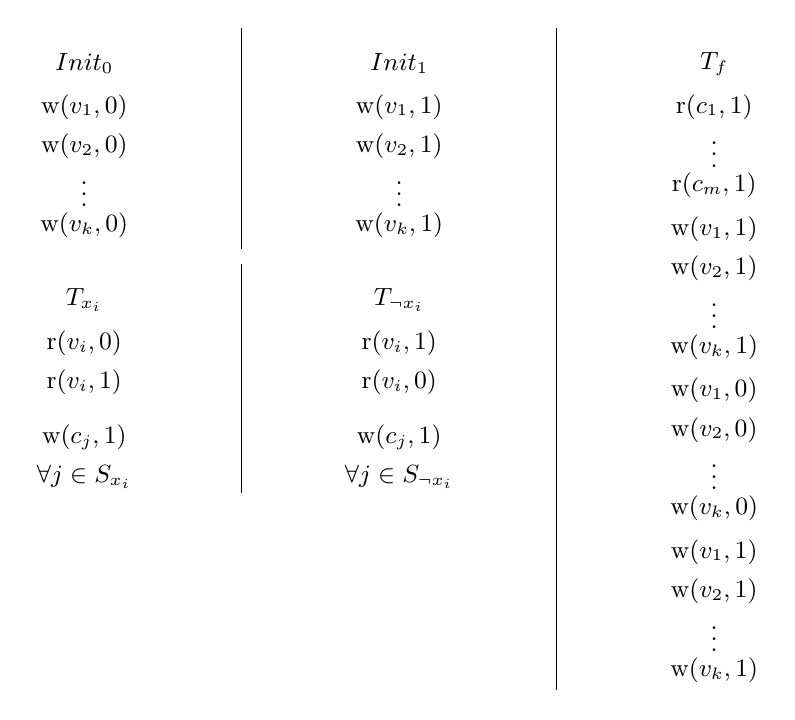
\begin{tikzpicture}[
    every node/.style={font=\small}
]

% =========================================================
% Init_0
% =========================================================

\node at (0,0) {$Init_0$};

\node at (0,-0.55) {$\mathrm{w}(v_1,0)$};
\node at (0,-1.05) {$\mathrm{w}(v_2,0)$};
\node at (0,-1.55) {$\vdots$};
\node at (0,-2.05) {$\mathrm{w}(v_k,0)$};


% =========================================================
% Init_1
% =========================================================

\node at (4.0,0) {$Init_1$};

\node at (4.0,-0.55) {$\mathrm{w}(v_1,1)$};
\node at (4.0,-1.05) {$\mathrm{w}(v_2,1)$};
\node at (4.0,-1.55) {$\vdots$};
\node at (4.0,-2.05) {$\mathrm{w}(v_k,1)$};


% =========================================================
% T_{x_i} -- below Init_0
% =========================================================

\node at (0,-3.0) {$T_{x_i}$};

\node at (0,-3.55) {$\mathrm{r}(v_i,0)$};
\node at (0,-4.05) {$\mathrm{r}(v_i,1)$};

\node at (0,-4.75) {$\mathrm{w}(c_j,1)$};
\node at (0,-5.25) {$\forall j\in S_{x_i}$};


% =========================================================
% T_{\neg x_i} -- below Init_1
% =========================================================

\node at (4.0,-3.0) {$T_{\neg x_i}$};

\node at (4.0,-3.55) {$\mathrm{r}(v_i,1)$};
\node at (4.0,-4.05) {$\mathrm{r}(v_i,0)$};

\node at (4.0,-4.75) {$\mathrm{w}(c_j,1)$};
\node at (4.0,-5.25) {$\forall j\in S_{\neg x_i}$};


% =========================================================
% T_f
% =========================================================

\node at (8.0,0) {$T_f$};

\node at (8.0,-0.55) {$\mathrm{r}(c_1,1)$};
\node at (8.0,-1.05) {$\vdots$};
\node at (8.0,-1.55) {$\mathrm{r}(c_m,1)$};

\node at (8.0,-2.10) {$\mathrm{w}(v_1,1)$};
\node at (8.0,-2.60) {$\mathrm{w}(v_2,1)$};
\node at (8.0,-3.10) {$\vdots$};
\node at (8.0,-3.60) {$\mathrm{w}(v_k,1)$};

\node at (8.0,-4.15) {$\mathrm{w}(v_1,0)$};
\node at (8.0,-4.65) {$\mathrm{w}(v_2,0)$};
\node at (8.0,-5.15) {$\vdots$};
\node at (8.0,-5.65) {$\mathrm{w}(v_k,0)$};

\node at (8.0,-6.20) {$\mathrm{w}(v_1,1)$};
\node at (8.0,-6.70) {$\mathrm{w}(v_2,1)$};
\node at (8.0,-7.20) {$\vdots$};
\node at (8.0,-7.70) {$\mathrm{w}(v_k,1)$};


% =========================================================
% Vertical separators
% =========================================================

\draw (2.0,0.45) -- (2.0,-2.35);
\draw (2.0,-2.55) -- (2.0,-5.45);
\draw (6.0,0.45) -- (6.0,-7.95);

\end{tikzpicture}
\caption{Threads in the reduction for $\rlxmm$}
    \label{tab:reduction-threads-relaxed}
\end{figure}

The threads $\mathsf{Init}{1}$ and $\mathsf{Init}{0}$ initialize the valuation used to evaluate the formula. For each variable $x_i$ corresponding to the Boolean variables of $\varphi$, $\mathsf{Init}{1}$ writes $1$ and $\mathsf{Init}{0}$ writes $0$. 
$T_{x_i}$ has a read statement $\rd(v_i,0)$ followed by $\rd(v_i,1)$ (which denotes reading \emph{true} for $x_i$) and sets all clauses containing $x_i$ to true, using the statement $\wt(c_j, 1)$ for all $j \in S_{x_i}$. 


Similarly, thread $T_{\neg x_i}$ reads $\rd(v_i, 1)$ followed by $\rd(v_i, 0)$ (denoting the value \emph{false} for $x_i$) and sets all clauses containing $\neg x_i$ to true. 
Finally the thread $T_{f}$ needs to make sure that all clauses are set to true, accomplished by the read statements $\rd(c_1, 1), \dots, \rd(c_m, 1)$.
Then, $T_{f}$ proceeds through the following steps (1) all the variables $v_i$s are set to $0$, followed by (2) setting all the variables $v_i$s to $1$, and finally (3) setting all the variables $v_i$s to $0$ again.
This sequence ensures that any threads $T_{x_i}$, $T_{\neg x_i}$ which were not executed in Phase 2 now have their conditions satisfied and can complete their execution. 
%%%%%%%%%

\begin{table}[h]
    
\noindent
\begin{minipage}{0.45\textwidth}
\centering
\begin{tabular}{c | c}
    $Init_0$ & $Init_1$ \\
    $\wt(v_1,0)$~& ~$\wt(v_1,1)$ \\ 
    $\wt(v_2,0)$~& ~$\wt(v_2,1)$ \\ 
    $\wt(v_3,0)$~& ~$\wt(v_3,1)$ \\

\end{tabular}
\vspace{.1cm}

\begin{tabular}{c | c}
    $T_{x_1}$ & $T_{\neg x_1}$ \\
    $\rd(v_1,0)$~& ~$\rd(v_1,1)$ \\ 
    $\rd(v_1,1)$~& ~$\rd(v_1,0)$ \\ 
    $\wt(c_1, 1)$~& ~ \\
    $\wt(c_2,1)$~&~ \\
\end{tabular}
\vspace{.1cm}

\begin{tabular}{c | c}
    $T_{x_2}$ & $T_{\neg x_2}$\\
     $\rd(v_2,0)$~& ~$\rd(v_2,1)$ \\ 
    $\rd(v_2,1)$~& ~$\rd(v_2,0)$ \\ 
    $\wt(c_2, 1)$~& ~ $\wt(c_2,1)$\\
\end{tabular}
\vspace{.1cm}

\begin{tabular}{c | c}
    $T_{x_3}$ & $T_{\neg x_3}$\\
     $\rd(v_3,0)$~& ~$\rd(v_3,1)$ \\ 
    $\rd(v_3,1)$~& ~$\rd(v_3,0)$ \\ 
    $\wt(c_2, 1)$~& ~ $\wt(c_2,1)$\\
   
\end{tabular}

\end{minipage}
\hfill
\begin{minipage}{0.45\textwidth}
\centering
\begin{tabular}{c}
    $T_f$ \\
     $\rd(c_1, 1)$ \\
    $\rd(c_2, 1)$ \\
    $\wt(v_1, 1)$ \\
    $\wt(v_2, 1)$ \\
    $\wt(v_3, 1)$ \\
    $\wt(v_1, 0)$ \\
    $\wt(v_2, 0)$ \\
    $\wt(v_3, 0)$ \\
    $\wt(v_1, 1)$ \\
    $\wt(v_2, 1)$ \\
    $\wt(v_3, 1)$ \\

\end{tabular}
\end{minipage}
\vspace{2em}
\caption{$\varphi=(x_1\lor x_2\lor x_3)\land (x_1 \lor \neg x_2\lor \neg x_3)$}
    \label{tab:relaxed-example-finegrainedwra}
\end{table}
%%%%%%%%%%%%%%%%

\begin{lemma}
    $\varphi$ is satisfiable iff $\expartial_\varphi  \models \rlxmm$.
\end{lemma}

\begin{proof}
    Suppose $A$ is a satisfying assignment for $\varphi$. We explictly describe the $\rf$ relation and $\mo$ relation as follows. 
    
    If $A(x_i) = true$:
    \begin{itemize}[leftmargin=0.1em]
    \item $\tuple{Init_0: \wt(v_i, 0)}~\rf~\tuple{T_{x_i}: \rd(v_i, 0)}$ and $\tuple{Init_1: \wt(v_i, 1)}~\rf~\tuple{T_{x_i}: \rd(v_i, 1)}$,
    \item $\tuple{T_f: \wt(v_i, 1)}~\rf~\tuple{T_{\neg x_i}: \rd(v_i, 1)}$, and $\tuple{T_f: \wt(v_i, 0)}~\rf~\tuple{T_{\neg x_i}: \rd(v_i, 0)}$. 
    \end{itemize} 
    Else, when $A(x_i) = false$, 
    \begin{itemize}[leftmargin=0.1em]
    \item $\tuple{Init_1: \wt(v_i, 1)}~\rf~\tuple{T_{\neg x_i}: \rd(v_i, 1)}$, and $\tuple{Init_0: \wt(v_i, 0)}~\rf~\tuple{T_{\neg x_i}: \rd(v_i, 0)}$,
    \item $\tuple{T_f: \wt(v_i, 0)}~\rf~\tuple{T_{ x_i}: \rd(v_i, 0)}$, and $\tuple{T_f: \wt(v_i, 1)}~\rf~\tuple{T_{ x_i}: \rd(v_i, 1)}$. 
    \end{itemize} 
            
    Coming to variables $c_i$s, for each $T_f: \rd(c_j, 1)$ there is a literal $\ell_j$ in clause $C_j$ that is true. Let $\tuple{T_{\ell_j}: \wt(c_j, 1)}~\rf~ \tuple{T_f: \rd(c_j, 1)}$. Observe that the constructed $\rf$ satisfies $\po-\rf$-acyclicity.
    
    The $\rf$ induces the following $\mo$ relation. If $A(x_i) = true$: 
    \begin{itemize}[leftmargin=0.1em]
    \item $\tuple{Init_0: \wt(v_i, 0)} ~\mo~\tuple{Init_1: \wt(v_i, 1)} ~\mo~\tuple{T_f: \wt(v_i, 1)}~\mo~\tuple{T_f: \wt(v_i, 0)} ~\mo~\\ \tuple{T_f: \wt(v_i, 1)}$
    \item For each clause $C_j$ there are three threads writing $\wt(c_j, 1)$.  For $C_j$, choose a specific literal $\ell_j$ that is made true by the satisfying assignment $A$. 
    The $\mo$ relation orders the write statements $\wt(c_j, 1)$ in literals that are set to true before $T_{\ell_j}: \wt(c_j, 1)$, and those in literals that set to false after $T_{\ell_j}: \wt(c_j, 1)$.
    \end{itemize}  
    When $A(x_i) = false$, an $\mo$ order can be defined analogously. 
    
    \begin{figure*}% 
\begin{center}
 \begin{tikzpicture}[scale =1,yscale=2, 
    op/.style={draw, fill=white, rounded corners, minimum width=1.25cm, minimum height=0.55cm, 
               inner sep=2pt, font=\small},
    thread/.style={font=\small\bfseries},
    >=stealth
]

% ------------------------------------------------------------
% First group: T_i^1 and T_i^0
% ------------------------------------------------------------

% Init_0 / Init_1
\node[thread] (T11) at (0, 0.9) {$Init_0$};
\node[thread] (T10) at (2.0, 0.9) {$Init_1$};

\node[op] (i01) at (0, 0.2) {$\wt(v_1,0)$};
\node[op] (i02) at (0,-0.5) {$\wt(v_2,0)$};
\node[op] (i03)  at (0,-1.2) {$\wt(v_3,0)$};

\draw[po] (i01) to (i02);
\draw[po] (i02) to (i03);



\node[op] (i11) at (2.0, 0.2) {$\wt(v_1,1)$};
\node[op] (i12) at (2.0,-0.5) {$\wt(v_2,1)$};
\node[op] (i13)  at (2.0,-1.2) {$\wt(v_3,1)$};


\draw[po] (i11) to (i12);
\draw[po] (i12) to (i13);

\draw[mo] (i01) to node[above] {\footnotesize$\mo$} (i11);
\draw[mo] (i12) to node[above] {\footnotesize$\mo$} (i02);
\draw[mo] (i13) to node[above] {\footnotesize$\mo$} (i03);

% T_2^1 / T_2^0

% ------------------------------------------------------------
% Second group: T_xi and T_not xi
% ------------------------------------------------------------

% T_x1 / T_not x1
\node[thread] (Tx1)  at (5.0, 1.3) {$T_{x_1}$};
\node[thread] (Tnx1) at (7.0, 1.3) {$T_{\neg x_1}$};

\node[op] (v10) at (5.0,0.9) {$\rd(v_1,0)$};
\node[op] (v11) at (5.0,0.2) {$\rd(v_1,1)$};

\node[op] (c11)  at (5.0,-0.5) {$\wt(c_1,1)$};
\node[op] (c21)  at (5.0,-1.2) {$\wt(c_2,1)$};

\draw[po] (v10) to (v11);
\draw[po] (v11) to (c11);
\draw[po] (c11) to (c21);
\draw[rf] (i01) to node[above right] {\footnotesize$\rf$} (v10);
\draw[rf] (i11) to node[above right] {\footnotesize$\rf$} (v11);

\node[op] (v'11) at (7.0,0.9) {$\rd(v_1,1)$};
\node[op] (v'10) at (7.0,0.2) {$\rd(v_1,0)$};
\draw[po] (v'11) to (v'10); 

% T_x2 / T_not x2
\node[thread] (Tx2)  at (5.0,-2) {$T_{x_2}$};
\node[thread] (Tnx2) at (7.0,-2) {$T_{\neg x_2}$};

\node[op] (v20) at (5.0,-2.4) {$\rd(v_2,0)$};
\node[op] (v21) at (5.0,-3.1) {$\rd(v_2,1)$};
\node[op] (c12)  at (5.0,-3.8) {$\wt(c_1,1)$};

\draw[po] (v20) to (v21);
\draw[po] (v21) to (c12);

\node[op] (v'21) at (7.0,-2.4) {$\rd(v_2,1)$};
\node[op] (v'20) at (7.0,-3.1) {$\rd(v_2,0)$};
\node[op] (c22)  at (7.0,-3.8) {$\wt(c_2,1)$};

\draw[po] (v'21) to (v'20);
\draw[po] (v'20) to (c22);

% T_x3 / T_not x3
\node[thread] (Tx3)  at (5.0,-4.6) {$T_{x_3}$};
\node[thread] (Tnx3) at (7.0,-4.6) {$T_{\neg x_3}$};

\node[op] (v30) at (5.0,-5) {$\rd(v_3,0)$};
\node[op] (v31) at (5.0,-5.7) {$\rd(v_3,1)$};
\node[op] (c13)  at (5.0,-6.4) {$\wt(c_1,1)$};
\draw[po] (v30) to (v31);
\draw[po] (v31) to (c13);

\node[op] (v'31) at (7.0,-5) {$\rd(v_3,1)$};
\node[op] (v'30) at (7.0,-5.7) {$\rd(v_3,0)$};
\node[op] (c23)  at (7.0,-6.4) {$\wt(c_2,1)$};
\draw[po] (v'31) to (v'30);
\draw[po] (v'30) to (c23);

\draw[mo, bend right=45] (c11) to (c12.west);
\draw[mo, bend left=5] (c22.west) to (c21.east);
\draw[mo, bend right=50] (c11.west) to (c13.west);
\draw[mo, bend right=70] (c23.east) to (c21.east);

% ------------------------------------------------------------
% Final thread T_f
% ------------------------------------------------------------

\node[thread] (Tf) at (10.0,0.9) {$T_f$};

\node[op] (fc1) at (10.0,0.2) {$\rd(c_1,1)$};
\node[op] (fc2) at (10.0,-0.5) {$\rd(c_2,1)$};
\node[op] (fv11) at (10.0,-1.2) {$\wt(v_1,1)$};
\node[op] (fv21) at (10.0,-1.9) {$\wt(v_2,1)$};
\node[op] (fv31) at (10.0,-2.6) {$\wt(v_3,1)$};
\node[op] (fv10) at (10.0,-3.3) {$\wt(v_1,0)$};
\node[op] (fv20) at (10.0,-4.0) {$\wt(v_2,0)$};
\node[op] (fv30) at (10.0,-4.7) {$\wt(v_3,0)$};
\node[op] (fv'11) at (10.0,-5.4) {$\wt(v_1,1)$};
\node[op] (fv'21) at (10.0,-6.1) {$\wt(v_2,1)$};
\node[op] (fv'31) at (10.0,-6.8) {$\wt(v_3,1)$};

%po for Tf
\draw[po] (fc1) to (fc2);
\draw[po] (fc2) to (fv11);
\draw[po] (fv11) to (fv21);
\draw[po] (fv21) to (fv31);
\draw[po] (fv31) to (fv10);
\draw[po] (fv10) to (fv20);
\draw[po] (fv20) to (fv30);
\draw[po] (fv30) to (fv'11);
\draw[po] (fv'11) to (fv'21);
\draw[po] (fv'21) to (fv'31);

%rf edges

\draw[rf] (c11) to node[above right] {\footnotesize$\rf$} (fc1);
\draw[rf] (c21) to node[above left] {\footnotesize$\rf$} (fc2);
\draw[rf, bend left=10] (fv11) to node[below right] {\footnotesize$\rf$} (v'11);
\draw[rf, bend left=20] (fv10) to node[above left] {\footnotesize$\rf$} (v'10);


%\draw[rf, bend right=8] (s11b) to (fs12);
%\draw[rf, bend right=25] (s10a) to (fs11);
%\draw[rf, bend left=10] (s20b) to (fs22);
%\draw[rf, bend left=10] (s21a) to (fs21);
%\draw[rf, bend left=0] (s30b) to (fs32);
%\draw[rf, bend left=0] (s31a) to (fs31);
\end{tikzpicture}%
\end{center}
\caption{Execution graph for Table~\ref{tab:relaxed-example-finegrainedwra}: The graph is restricted to the $\mo$-edges between writes of $Init_1$ and $Init_0$ and all synthesized  edges involving $v_1$}
\label{example-Execution-relaxed}
\end{figure*}%

    
    Table~\ref{tab:relaxed-example-finegrainedwra} gives an instance of the construction of $\expartial$ for the fine-grained hardness reduction for \threewriter~ and (Figure~\ref{example-Execution-relaxed}) shows the synthesis of $\rf$ and $\mo$-edges. To keep the figure simple, and less confusing we have only showed the synthesized edges related to $v_1$. The execution graph is constructed for $x_1=1, x_2=0, x_3=0$, a satisfying assignment for $\varphi$. The $\rf$ and $\mo$-edges follow the rules of construction we just discussed. 
    
    

    \paragraph*{Relaxed Write-coherence.} From our construction, it is easy to see $\irr(\mo_x; \po)$.

    \paragraph*{Relaxed Read-coherence.} We need to prove  $\irr(\rf^{-1}; \mo_x; \rf^{?}; \po)$. 
    If relaxed read coherence is violated, the violating pattern is of the following form there are read events $r_1$ and $r_2$, and two write events $w_1, w_2$ such that $w_1~\rf~r_1$, $w_2~\rf~r_2$, $w_1~\mo~w_2$ and $r_2~\po~r_1$.
    Such a violation can potentially happen on variables which have multiple read events in the same thread, which is only the case for $v_i$.
    We consider the various possibilities below. 
    We consider the case $A(x_i) = true$ below. 
        \begin{itemize}[leftmargin=0.1em]
            \item $\tuple{T_{x_i}: \rd(v_i, 0)} \po \tuple{T_{x_i}: \rd(v_i, 1)}$, reads-from $Init_0$ and $Init_1$ respectively, where $\mo$ agrees with the $\po$.
            \item $\tuple{T_{\neg x_i}: \rd(v_i, 1)} \po \tuple{T_{\neg x_i}: \rd(v_i, 0)}$, reads-from the first two writes on $v_i$ in $T_f$ respectively, where, once again $\mo$ agrees with the $\po$, and irreflexivity is ensured.
        \end{itemize}
        A similar argument can be made for the case the case $A(x_i) = false$.

    This shows that the constructed $\rf$ and $\mo$ are consistent with $\rlxmm$. 
    
    
    
    Conversely, suppose $\expartial_\varphi \models \rlxmm$. 
    We need to show that there are no two $\rd(c_j, 1)$ and $\rd(c_\ell, 1)$ reading from some $T_{x_i}$ and $T_{\neg x_i}$.
    Suppose not. 
    Let $\rd(c_j, 1)$ read from $T_{x_i}: \wt(c_j, 1)$ and $\rd(c_\ell, 1)$ read from $T_{\neg x_i}: \wt(c_\ell, 1)$.    
    Consider the thread $T_{x_i}$. Since $T_{x_i}: \wt(c_j, 1)$ has been read from, this means that the preceding read instructions of $T_{x_i}$ have been executed, and the only possible read from relation is as follows: 
    $\tuple{Init_0: \wt(v_i, 0)}~\rf~\tuple{T_{x_i}: \rd(v_i, 0)}$,
    and $\tuple{Init_1: \wt(v_i, 1)}~\rf~\tuple{T_{x_i}: \rd(v_i, 1)}$. 
    By relaxed read coherence axiom, this implies $\tuple{Init_0: \wt(v_i, 0)} ~\mo~\tuple{Init_1: \wt(v_i, 1)}$    

    Now, consider the thread $T_{\neg x_i}$. As argued fro $T_{x_i}$, since the last instruction has been read from, the preceding read instructions of $T_{x_i}$ have been executed with the only reads-from relation being 
    $\tuple{Init_1: \wt(v_i, 1)}~\rf~\tuple{T_{\neg x_i}: \rd(v_i, 1)}$ and $\tuple{Init_0: \wt(v_i, 0)}~\rf~\tuple{T_{\neg x_i}: \rd(v_i, 0)}$. 
    However, this violates relaxed read coherence axiom, as $\tuple{Init_0: \wt(v_i, 0)} ~\mo~\tuple{Init_1: \wt(v_i, 1)}$ but $\tuple{T_{\neg x_i}: \rd(v_i, 1)}~\po~\\ \tuple{T_{\neg x_i}: \rd(v_i, 0)}$. 
    This contradicts our assumption that there are two $\rd(c_j, 1)$ and $\rd(c_\ell, 1)$ reading from some $T_{x_i}$ and $T_{\neg x_i}$. 
    Thus, the assignment induced by the $T_i^b$ threads executed before $T_f$ satisfies $\varphi$.
\end{proof}

The above lemma prove Theorem~\ref{lem:relaxed-finegrained}.

In the next section we show that the $\vm$ problem is NP-hard for $\twowriter$. 

\section{NP-hardness for \twowriter\ systems}
\label{sec:np-relaxed}
Given a 3-CNF-SAT formula $\varphi$ with $k$ variables and $m$ clauses, we construct an abstract execution $\ypartial=(\E, \po)$ with $2k+m+3$ threads, accessing $k+2m+1$ memory locations $v_1, v_2, \dots, v_k, c_1, \dots, c_m, d_1, \dots, d_m, s$ and 2 values $0, 1$ such that $\varphi$ is satisfiable iff $\ypartial_\varphi^{\rlxmm}  \models \rlxmm$.
$\ypartial_\varphi^{\rlxmm}$ follows the general scheme depicted in Figure~\ref{fig:two-writer} of Chapter~\ref{RA-ptime}.

As in Section~\ref{sec:hardness-twowriter}, here also we face similar challenge of reducing the number of writers for $c_j$ to two. But besides this, we also need to reduce the number of writers for $v_i$'s. The former challenge is handled the same way as the $\twowriter$ construction in Section~\ref{sec:hardness-twowriter}. For the later challenge we do the following.
\begin{itemize}
 \item Remove all the writes from $T_f$ in $\expartial_{\varphi}$, and add it to $Init_1$ after $\wt(v_k,1)$. The order of the writes remain same as before.
 
\item So that the above writes can be executed only after $T_f$, add a $\wt(s,1)$ after the last read i $T_f$ and a $\rd(s,1)$ before newly the added  set of writes in $Init_1$.
\end{itemize}

The required changes to Table~\ref{tab:reduction-threads-relaxed} is reflected in Table~\ref{tab:np-reduction-threads-relaxed}

In this reduction also, a formula $\varphi$ with $k$ threads and $m$ clauses yields an execution graph with $\mathcal{O}(k + m)$ theads and this does not give the stronger hardness under ETH, parameterized by the number of threads. 

\begin{theorem}
\label{thm:relaxed-two-writer-hardness}
    The $\vm$ problem is $\NP$-complete for $\rlxmm$, even when restricted to \twowriter\ execution graphs.
\end{theorem}

The above theorem can be proved by the next two lemmas.

\begin{table}[h]
    
\noindent
\begin{minipage}{0.17\textwidth}
\centering
\begin{tabular}{c | c}
    $Init_0$ & $Init_1$ \\
    $\wt(v_1, 0)$~& ~$\wt(v_1, 1)$ \\
    $\wt(v_2, 0)$~ & ~$\wt(v_2, 1)$ \\
    $\cdots$ \\
    $\wt(v_k, 0)$~ & ~$\wt(v_k, 1)$\\
    & $\rd(s, 1)$ \\
    & $\wt(v_1, 0)$ \\
    & $\wt(v_2, 0)$ \\
    & $\cdots$ \\
    & $\wt(v_k, 0)$ \\
    & $\wt(v_1, 1)$ \\
    & $\wt(v_2, 1)$ \\
    & $\cdots$ \\
    & $\wt(v_k, 1)$ \\
    
\end{tabular}
\end{minipage}
\hfill
\begin{minipage}{0.35\textwidth}
\centering
\begin{tabular}{c | c}
    $T_{x_i}$~ & ~$T_{\neg x_i}$ \\
        $\rd(v_i, 0)$ ~&~  $\rd(v_i, 1)$ \\
        $\rd(v_i, 1)$ ~&~ $\rd(v_i, 0)$ \\
        & \\        
        $\wt(c_j, 1)$ ~&~ $\wt(c_j, 1)$ \\
        $\forall j \in S_{x_i}\setminus S_{x_i}^{3}$ ~&~  $\forall j \in S_{\neg x_i}\setminus S_{\neg x_i}^{3}$\\
        $\wt(d_j,1)$, $j\in S_{x_i}^{3}$~&~ $\wt(d_j,1)$, $j\in S_{\neg x_i}^{3}$\\
        \scriptsize $S_{x_i}^{3}=\{j:\ell_j^3=x_i\}$ ~&~  \scriptsize $S_{\neg x_i}^{3}=\{j:\ell_j^3=\neg x_i\}$
        
\end{tabular}
\end{minipage}
\hfill
\begin{minipage}{0.13\textwidth}
\centering
\begin{tabular}{c}
    $T_j$ \\
    $\rd(c_j, 1)$\\
    $\wt(d_j, 1)$ \\
    $\forall j \in \{1,\cdots,m\}$\\
\end{tabular}
\end{minipage}
\hfill
\begin{minipage}{0.13\textwidth}
\centering
\begin{tabular}{c}
    $T_f$ \\
    $\rd(d_1, 1)$ \\
    $\rd(d_2, 1)$ \\
    $\cdots$ \\
    $\rd(d_m, 1)$ \\
    $\wt(s, 1)$ \\
\end{tabular}
\end{minipage}
\vspace{2em}
\caption{Threads in the reduction for $\rlxmm$}
    \label{tab:np-reduction-threads-relaxed}
 %\vspace{-.8cm}   
\end{table}

\begin{lemma}
    $\varphi$ is satisfiable iff $\ypartial_\varphi^{\rlxmm}  \models \rlxmm$.
\end{lemma}

\begin{proof}
    Suppose $A$ is a satisfying assignment for $\varphi$. Then, the execution proceeds as follows. 
    The $\rf$ relation and $\mo$ relation are exactly as in Lemma~\ref{lem:relaxed-finegrained}, except the following.
    If $A(x_i) = true$:
    \begin{itemize}
        \item $\tuple{T_f: \wt(s, 1)}~\rf~\tuple{Init_1: \rd(s, 1)}$,
        \item $\tuple{Init_1: \wt(v_i, 1)}~\rf~\tuple{T_{\neg x_i}: \rd(v_i, 1)}$, and $\tuple{Init_1: \wt(v_i, 0)}~\rf~\tuple{T_{\neg x_i}: \rd(v_i, 0)}$. 
    \end{itemize} 
    For clause variables $c_j$ and $d_j$ , the $\rf$ (and consequently $\mo$) relation depends on the literals set to true by $A$. 
    For each clause $C_j$ there are two threads writing $\wt(c_j, 1)$, and two threads writing $\wt(d_j, 1)$. 
    
    If $A$ makes $\ell_j^3$ true then $\tuple{T_{\ell_j^3}: \wt(d_j, 1)}~\rf~\tuple{T_f: \rd(d_j, 1)}$. Otherwise $A$ makes $\ell_j^1$ or $\ell_j^2$ true. Let $\ell_j^k$ be the literal that is made true by the satisfying assignment $A$. Then, we have $\tuple{T_{\ell_j^k}: \wt(c_j, 1)}~\rf~\tuple{T_j: \rd(c_j, 1)}$ and $\tuple{T_j: \wt(d_j, 1)}~\rf~\tuple{T_f: \rd(d_j, 1)}$.

%    If $A$ makes $\ell_j^1$ or $\ell_j^2$ true, then $\tuple{T_{\ell_j^3}: \wt(d_j, 1)}~\rf~\tuple{T_f: \rd(d_j, 1)}$. Otherwise, $\tuple{T_j: \wt(d_j, 1)}~\rf~\tuple{T_f: \rd(d_j, 1)}$.
    For every variable-value pair for $c_j$ and $d_j$, there are atmost two writes. With the $\rf$ picked as above, the $\mo$ relation gets fixed: the unused write in $T_{x}$/ $T_{\neg x}$ that is set to true by $A$ is $\mo$-before the used write, while if the unused write is in $T_{x}$/ $T_{\neg x}$ that is set to false by $A$, then it is $\mo$-after the used write.    
    
    \paragraph*{Relaxed Write-coherence.} From our construction, it is easy to see $\irr(\mo_x; \po)$.
    %, which is easy to see from our construction. 

    \paragraph*{Relaxed Read-coherence.} We need to prove  $\irr(\rf^{-1}; \mo_x; \rf^{?}; \po)$. 
    The possible violating patterns and the arguments follow as in Lemma~\ref{lem:relaxed-finegrained}.

    This yields an $\rf$ where all $\rd(d_j, 1)$ in $T_f$ read from a thread corresponding to a true literal in $A$, so $\ypartial_\varphi^{\rlxmm} \models \rlxmm$.

    
    
    Conversely, suppose $\ypartial_\varphi^{\rlxmm} \models \rlxmm$. 
    The proof proceeds as in Lemma~\ref{lem:relaxed-finegrained}, where we show that if there are two clauses $C_j$ and $C_{\ell}$ such that $\rd(d_j, 1)$ and $\rd(c_\ell, 1)$ reading from some $T_{x_i}$ and $T_{\neg x_i}$, then relaxed read coherence is violated. .
\end{proof}


\section{Discussion}
We thus give similar trichotomy of results for the $\vm$-problem, as in case of $\ramm$-variants, with poynomial time for \onewriter{}, NP-Completenes for \twowriter{} and a fine-grained lower bound assuming ETH for \threewriter{}.  Note that we do not provide any conditional lower bound for relaxed as we did for $\ramm$ and their variants in Section~\ref{sec:1-writer-hardness} of Chapter~\ref{RA-ptime}. There we had reduced detecting triangle in a graph to the problem of consistency testing for $\onewriter$ systems under $\wramm$.  
To extend the construction to  Relaxed, \RlxRCoh should be violated on detecting a triangle. Violating relaxed-read-coherence needs either (i) two writes $\wt_1$, $\wt_2$ to a variable in different threads such that $\wt_1\mo\w$, are read by $\po$-related reads $\rd_1,~ \rd_2$ such that the $\po$-later
read reads from the mo-earlier write, or (ii) two writes $\wt_1$, $\wt_2$ in the same thread to a variable which
are read by po-related reads $\rd_1$, $\rd_2$ in the opposite order. (i) cannot be done with single-writer, while
(ii) violates relaxed-read-coherence irrespective of a triangle detection. So, it is not clear if such a superlinear lower bound exists for $\rlxmm$ and we keep it open. In the next chapter we prove similar type of results for the Causal Memory Models. We also provide the necessary axioms and examples to show how these models are related to the release-acquire fragment of C11. 




